\chapter*{Annexe A}
\markboth{\MakeUppercase{Annexe}}{}
\addcontentsline{toc}{chapter}{Annexe}
\adjustmtc
\thispagestyle{MyStyle}

%% add to table of contents : Annexe.1
\makeatletter\renewcommand\thesection{A.\@arabic\c@section}\makeatother

%add spacing in the table of figures
\addtocontents{lof}{\vspace{0.3cm}}
\appendix

\begin{figure}[H]
    \centering
    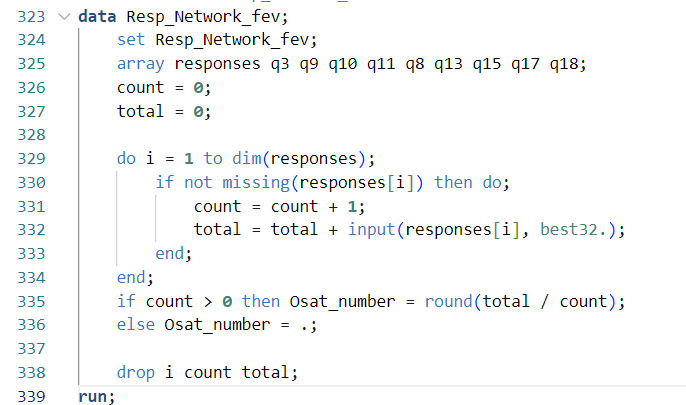
\includegraphics[width=0.6\linewidth]{capture_sas_1.png}
    \caption{Imputation de la colonne OSAT à partir de la moyenne des réponses aux questions}
    \label{imputation_code}
\end{figure}

\begin{figure}[H]
    \centering
    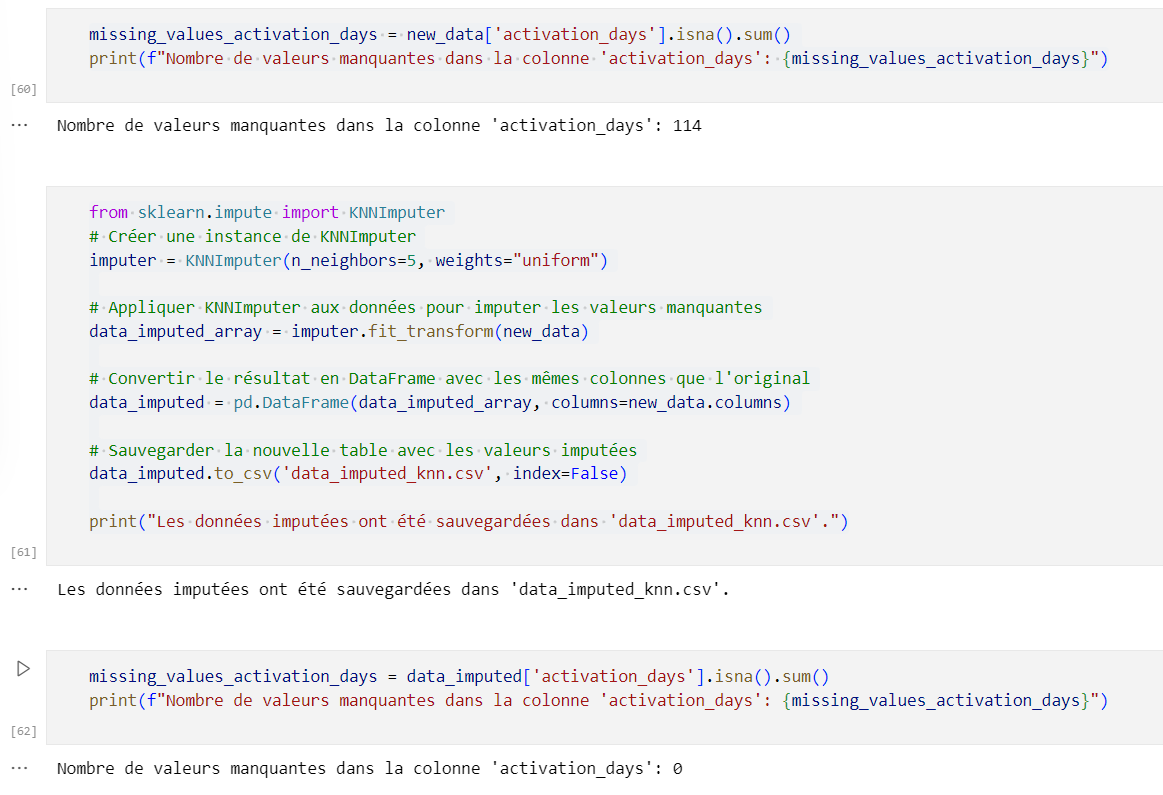
\includegraphics[width=0.8\linewidth]{capture_sas_6.png}
    \caption{Code pour l'imputation KNN}
    \label{fig:knn_code}
\end{figure}

\begin{figure}[H] 
    \centering 
    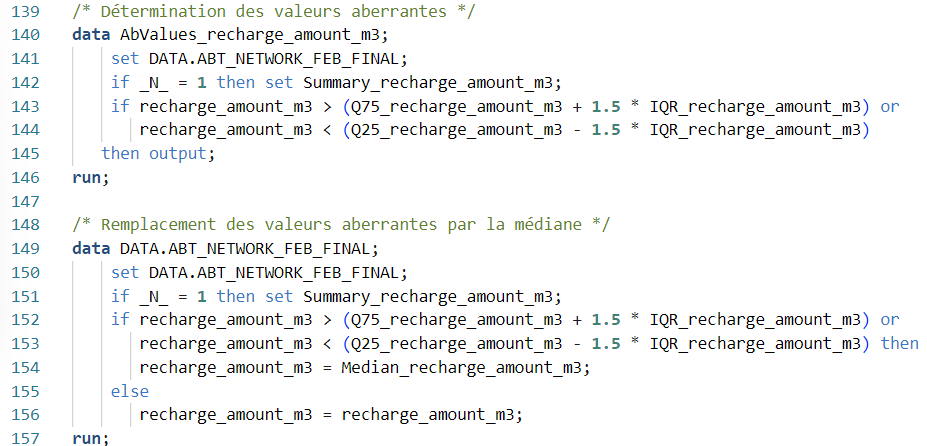
\includegraphics[width=0.7\linewidth]{capture_sas_7.png} 
    \caption{Remplacement des valeurs aberrantes par la médiane.}
    \label{fig:aberrant_values}
\end{figure}

\begin{figure}[H] 
    \centering 
    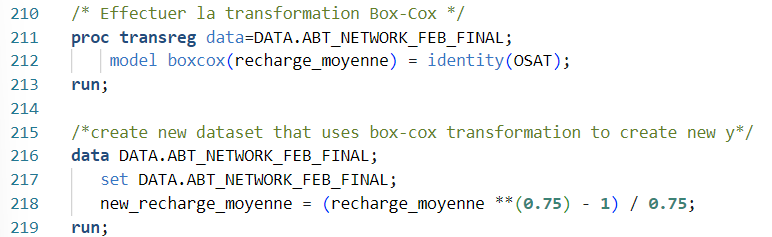
\includegraphics[width=0.7\linewidth]{capture_sas_9.png} 
    \caption{Transformation Box-Cox sur \textbf{Recharge\_moyenne}.}
    \label{fig:boxcox_transformation}
\end{figure}


\begin{figure}[H]
    \centering
    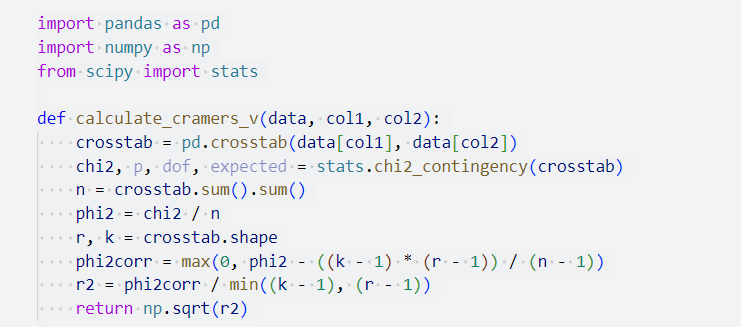
\includegraphics[width=0.8\linewidth]{capture_sas_12.png}
    \caption{Calcul de l'indice de Cramér’s V}
    \label{00}
\end{figure}
\vspace{10pt}

\begin{figure}[H]
    \centering
    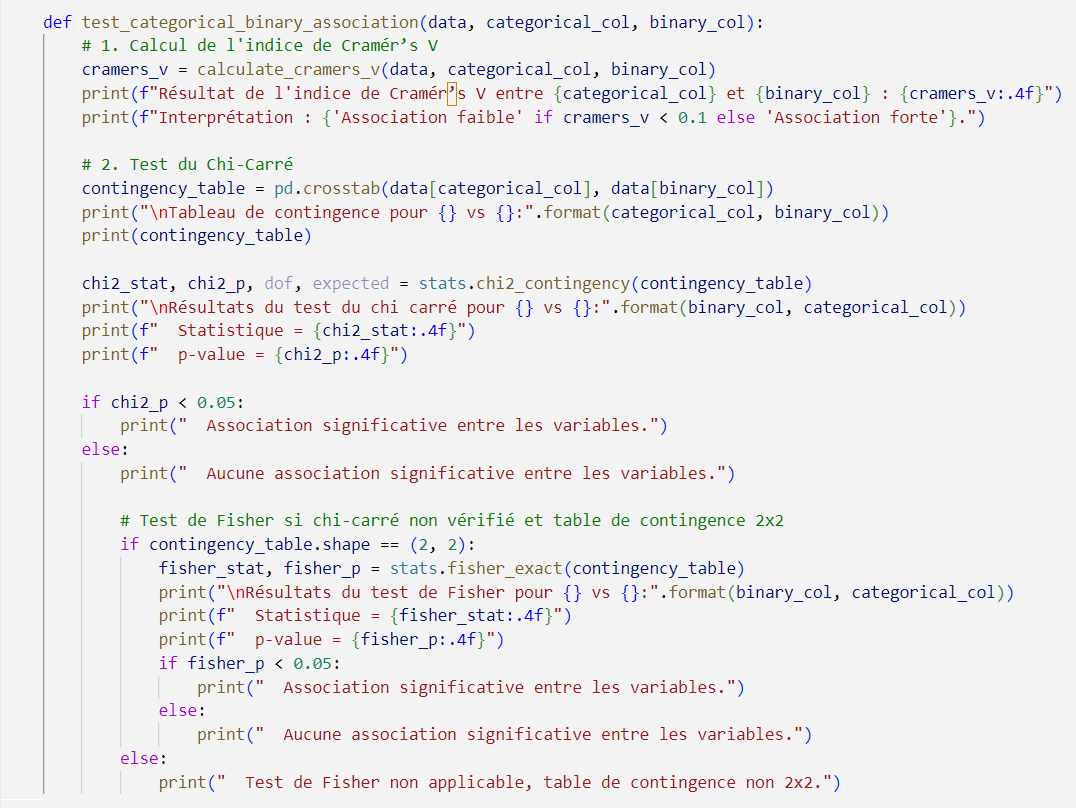
\includegraphics[width=\textwidth]{capture_sas_13.png}
    \caption{Test du Chi-Carré et test de Fisher (si applicable)}
    \label{222}
\end{figure}
\vspace{10pt}

\begin{figure}[H]
    \centering
    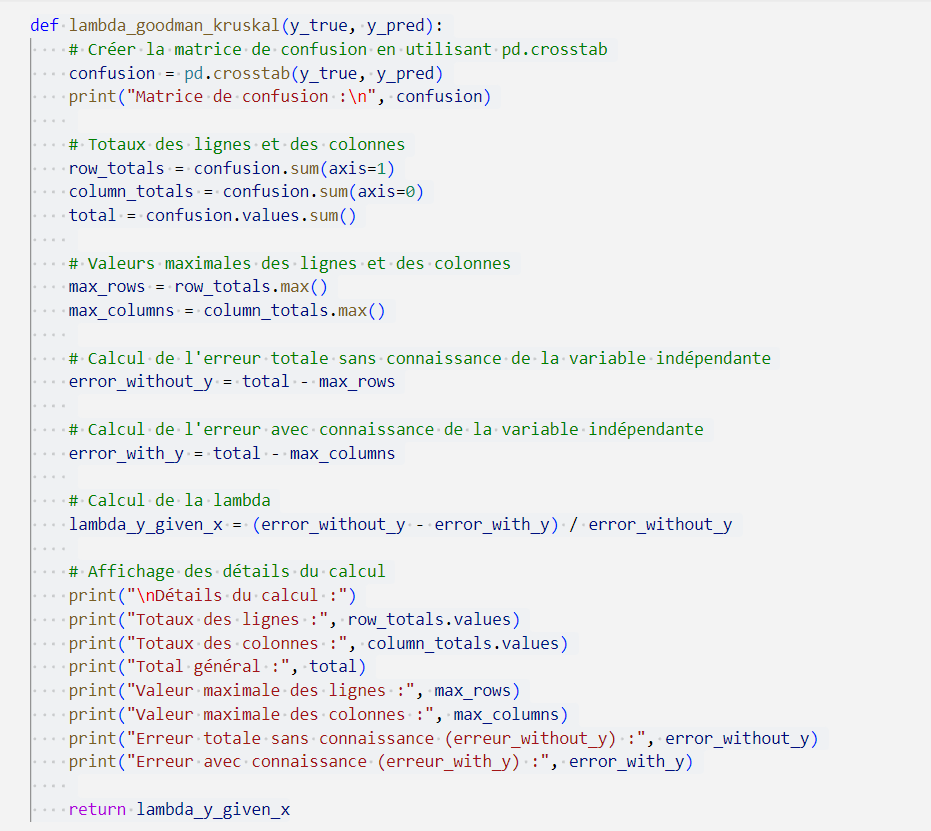
\includegraphics[width=\textwidth]{capture_sas_16.png}
    \caption{Calcul de la Lambda de Goodman et Kruskal}
    \label{555}
\end{figure}
\vspace{10pt}

\begin{figure}[H]
    \centering
    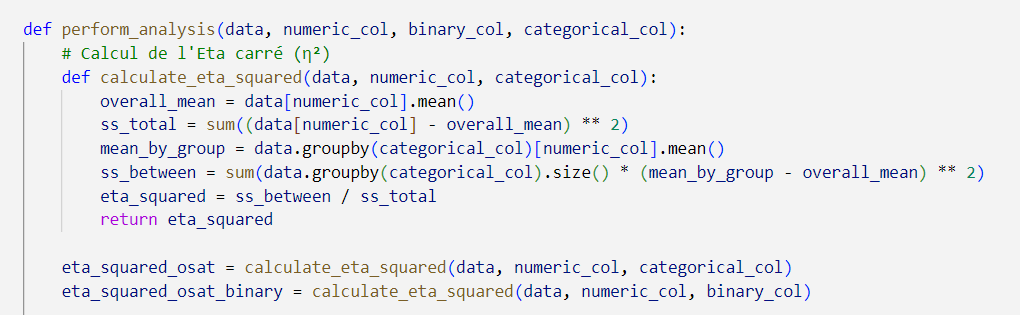
\includegraphics[width=0.9\textwidth]{capture_sas_19.png}
    \caption{Calcul de l'Eta carré pour \textbf{osat\_binary}}
    \label{26203}
\end{figure}
\vspace{10pt}

\begin{figure}[H]
    \centering
    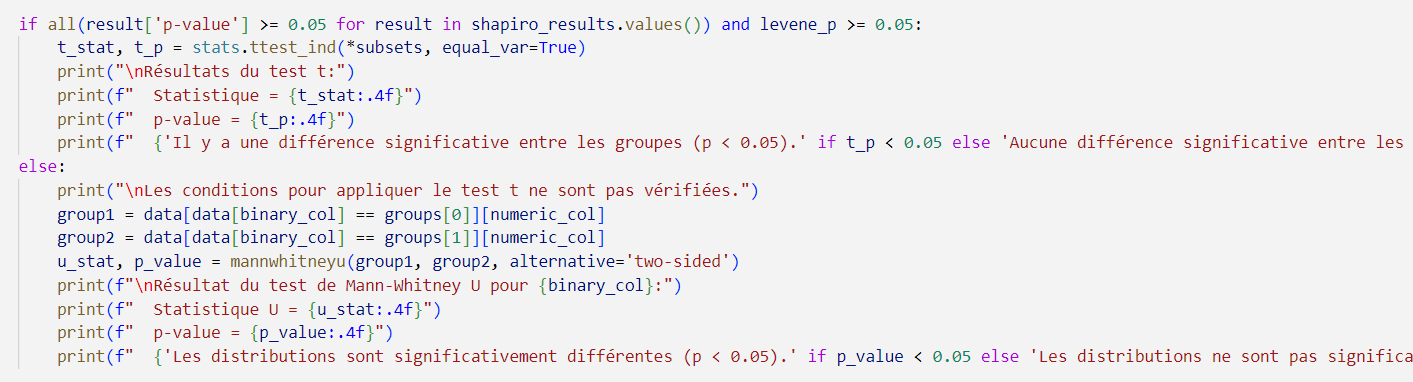
\includegraphics[width=0.8\linewidth]{capture_sas_21.png}
    \caption{Test d'homogénéité des variances de Levene}
    \label{168}
\end{figure}
\vspace{10pt}

\begin{figure}[H]
    \centering
    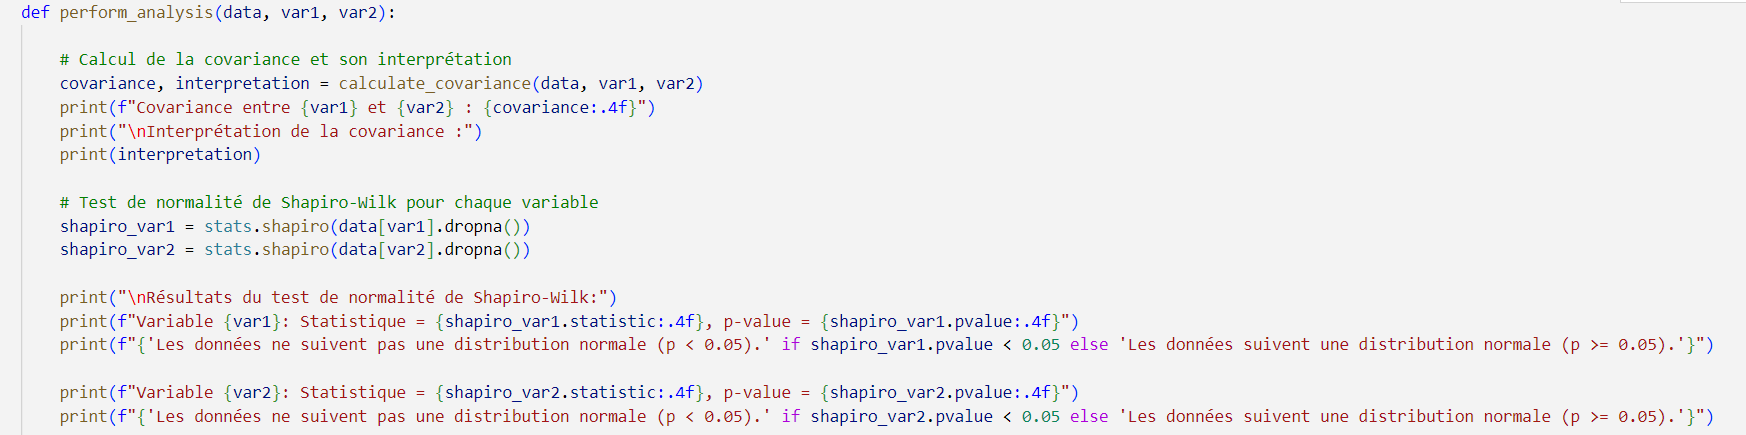
\includegraphics[width=0.8\linewidth]{capture_sas_28.png}
    \caption{Calcul de la covariance et test de normalité (Shapiro-Wilk) pour deux variables}
    \label{molka}
\end{figure}
\vspace{10pt}

\begin{figure}[H]
    \centering
    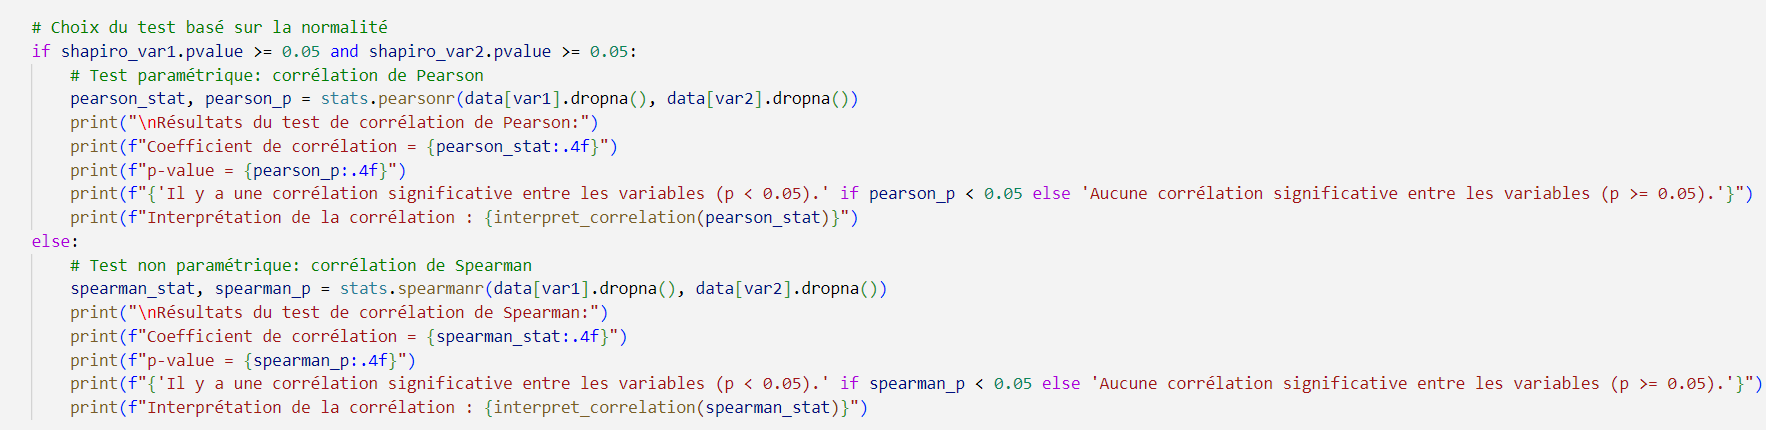
\includegraphics[width=0.8\linewidth]{capture_sas_29.png}
    \caption{Choix du test de corrélation: Pearson ou Spearman, basé sur la normalité des données}
    \label{hamma}
\end{figure}
\vspace{10pt}

\begin{figure}[H]
    \centering
    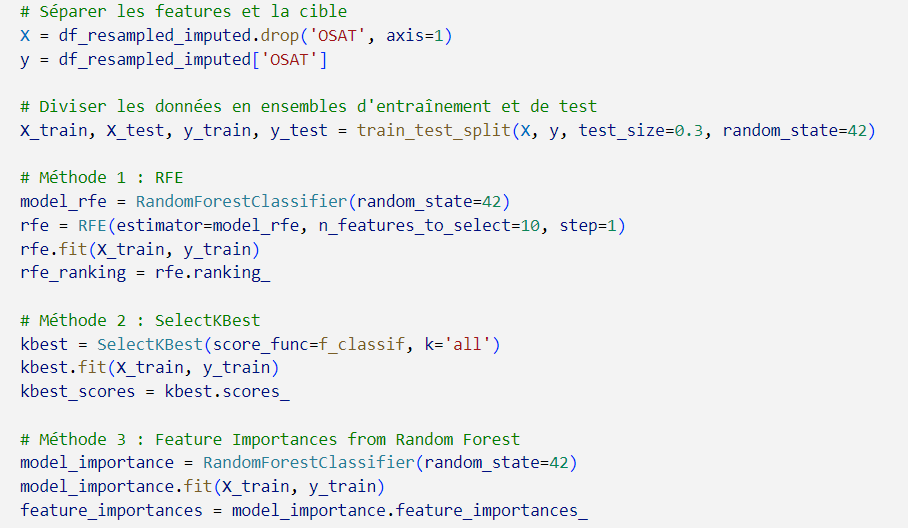
\includegraphics[width=0.9\linewidth]{capture_sas_61.png}
    \caption{Code de sélection des caractéristiques avec RFE, SelectKBest, et Random Forest}
    \label{code_features_Selection}
\end{figure}
\vspace{10pt}

\begin{figure}[H]
    \centering
    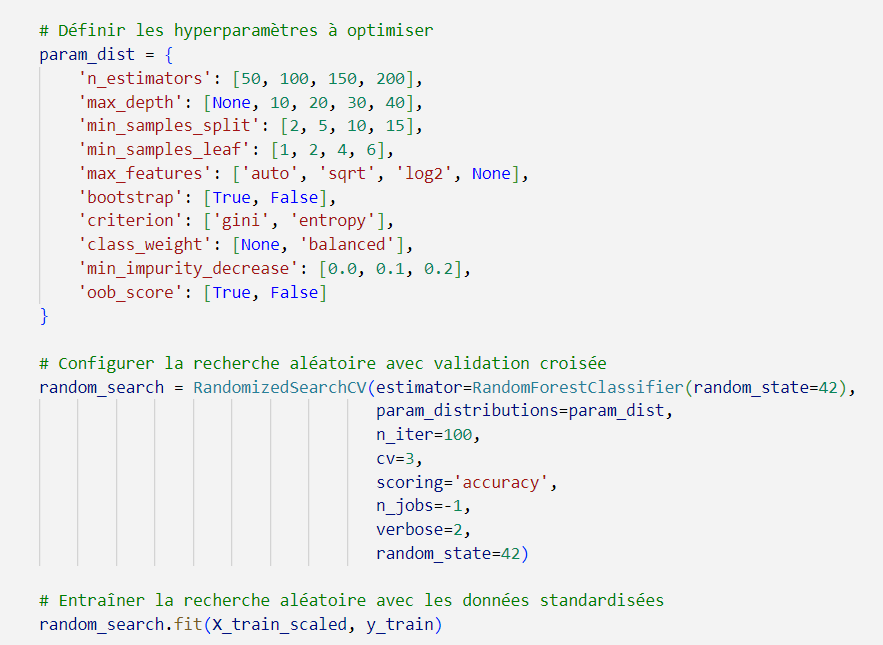
\includegraphics[width=0.9\linewidth]{capture_sas_70.png}
    \caption{Optimisation des hyperparamètres pour Random Forest}
    \label{hyperparametres}
\end{figure}
\vspace{10pt}

\begin{figure}[H]
    \centering
    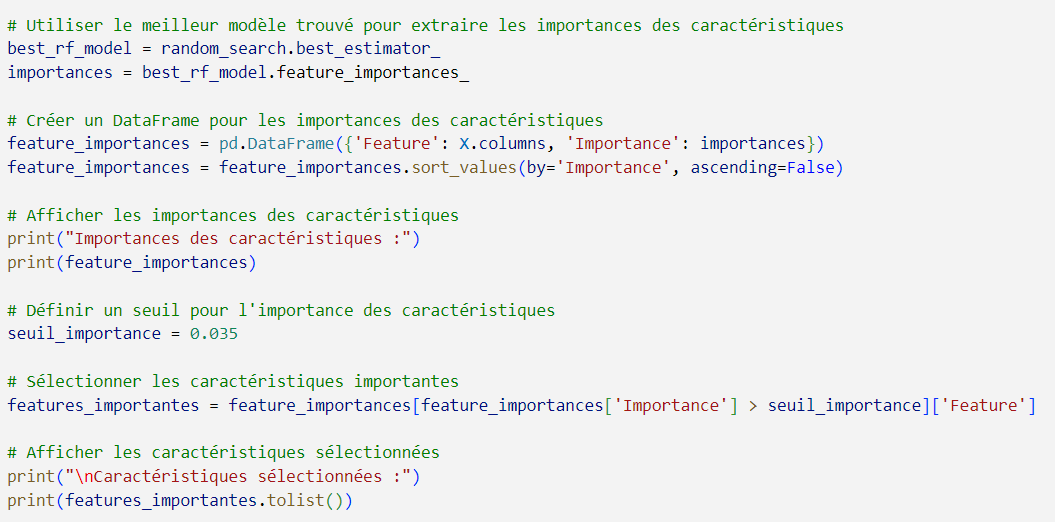
\includegraphics[width=0.9\linewidth]{capture_sas_71.png}
    \caption{Importances des caractéristiques par Random Forest}
    \label{importance}
\end{figure}
\vspace{10pt}

\begin{figure}[H]
    \centering
    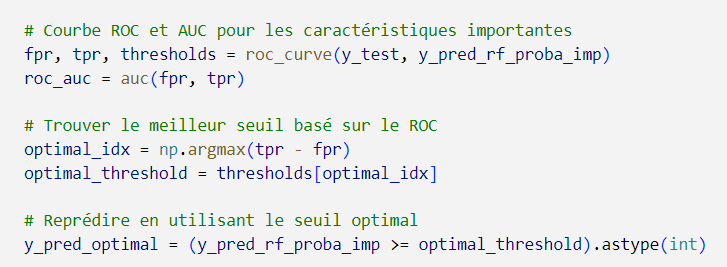
\includegraphics[width=0.7\linewidth]{capture_sas_72.png}
    \caption{Courbe ROC pour Random Forest avec AUC.}
    \label{code_roc}
\end{figure}
\vspace{10pt}

\begin{figure}[H]
    \centering
    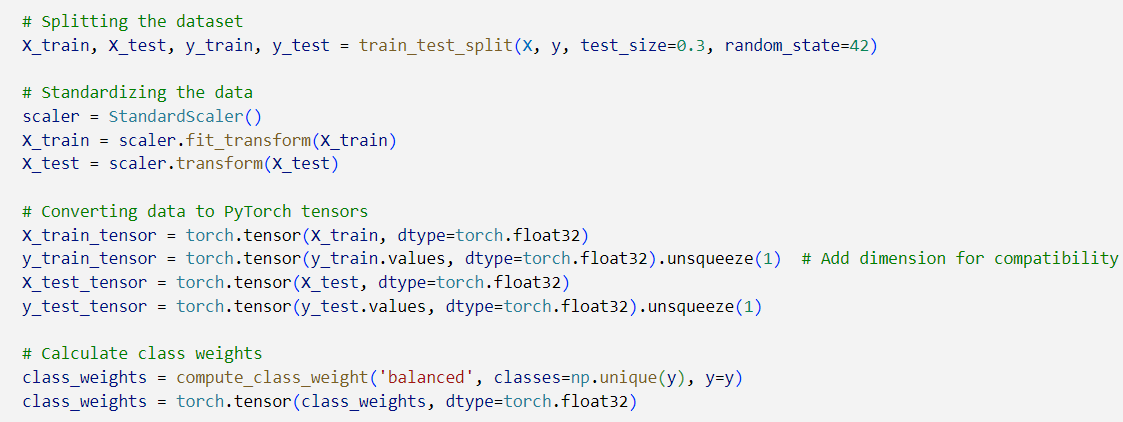
\includegraphics[width=0.9\linewidth]{capture_sas_73.png}
    \caption{Préparation des données pour PyTorch.}
    \label{pytorch_code}
\end{figure}
\vspace{10pt}

\begin{figure}[H]
    \centering
    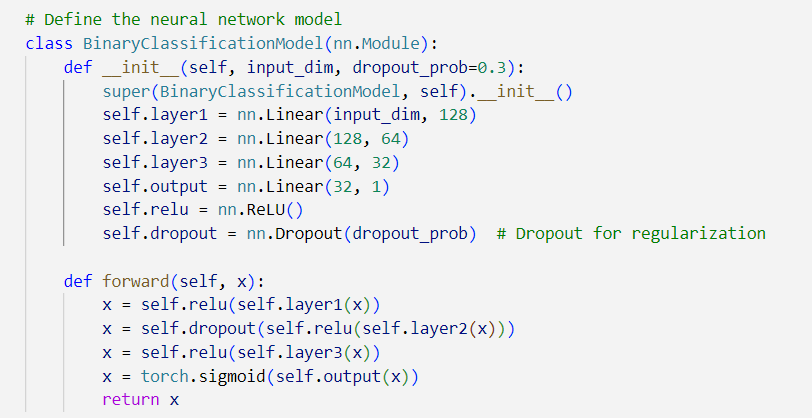
\includegraphics[width=0.8\linewidth]{capture_sas_74.png}
    \caption{Architecture du modèle de classification binaire dans PyTorch.}
    \label{model_architecture}
\end{figure}
\vspace{10pt}

\begin{figure}[H]
    \centering
    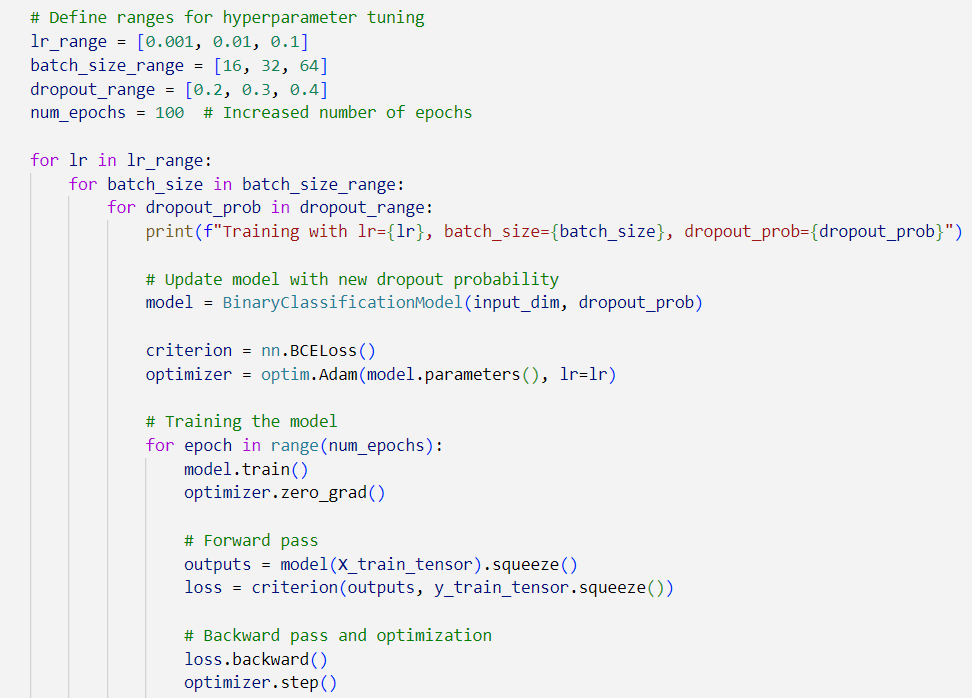
\includegraphics[width=0.8\linewidth]{capture_sas_75.png}
    \caption{Réglage des hyperparamètres pour le modèle PyTorch.}
    \label{fig_hyperparam_code}
\end{figure}
\vspace{10pt}

\begin{figure}[H]
    \centering
    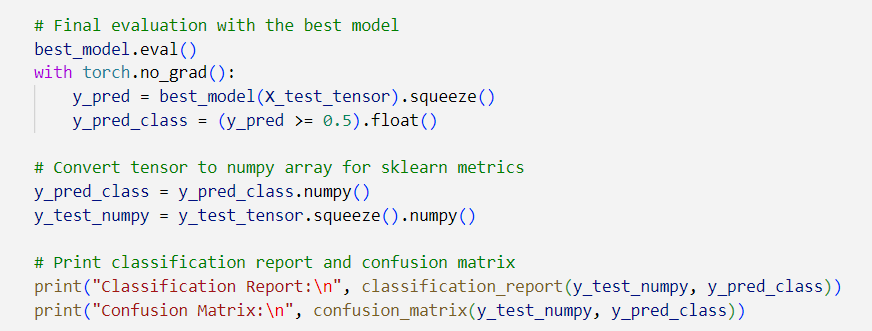
\includegraphics[width=0.8\linewidth]{capture_sas_77.png}
    \caption{Sélection du meilleur modèle PyTorch et évaluation finale.}
    \label{753}
\end{figure}
\vspace{10pt}

\begin{figure}[H]
    \centering
    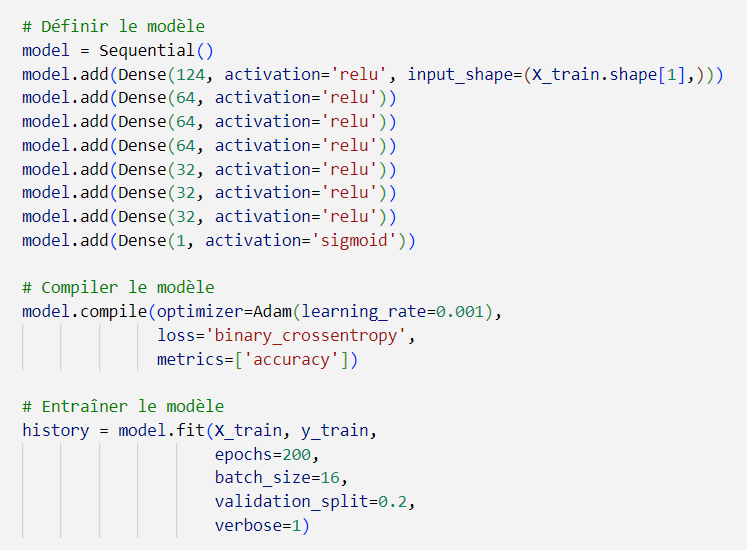
\includegraphics[width=0.7\linewidth]{capture_sas_78.png}
    \caption{Architecture classique du modèle Keras.}
    \label{96}
\end{figure}
\vspace{10pt}

\begin{figure}[H]
    \centering
    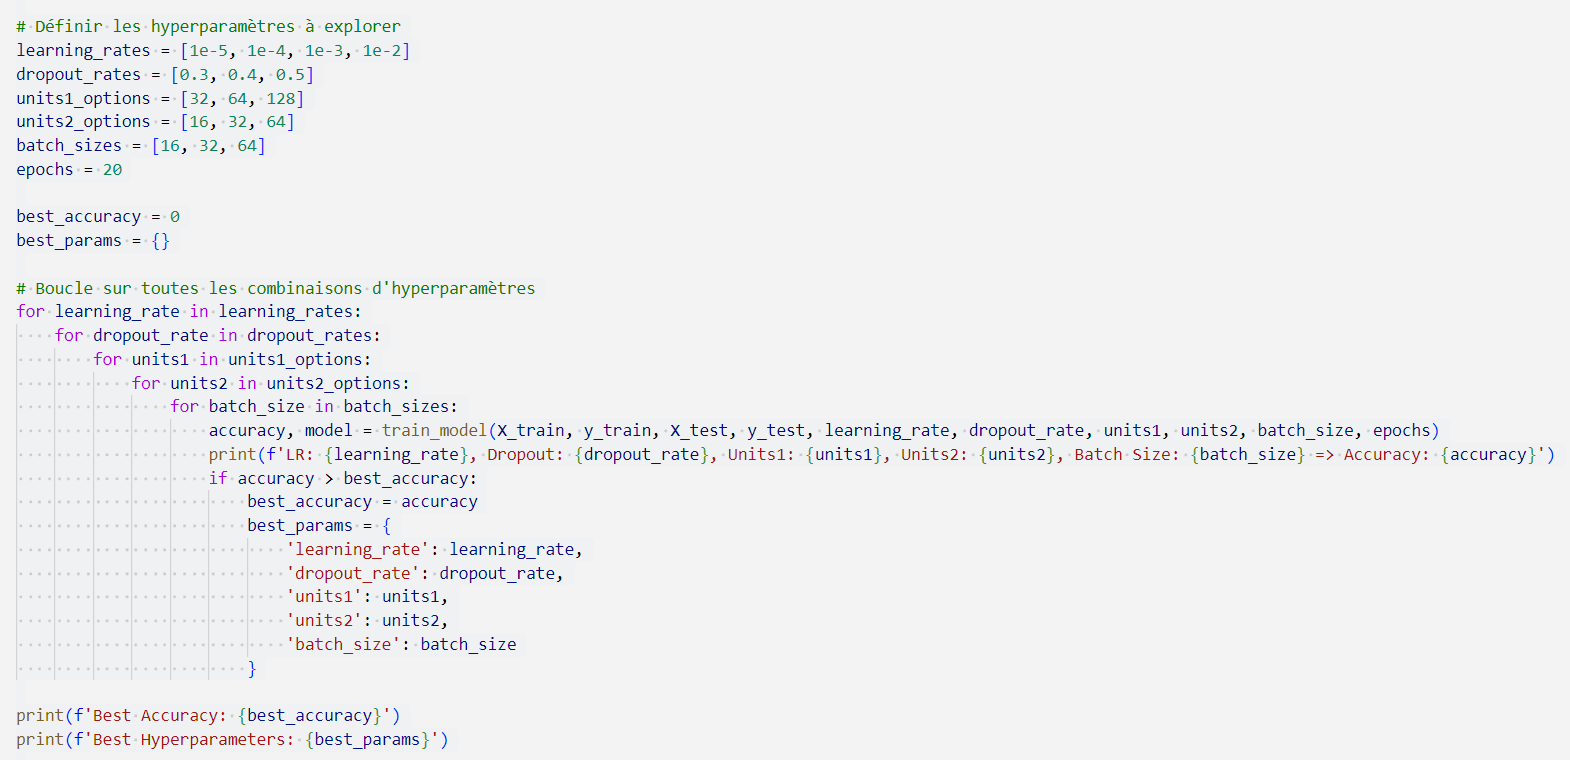
\includegraphics[width=0.9\linewidth]{capture_sas_79.png}
    \caption{Optimisation des hyperparamètres du modèle Keras.}
    \label{op}
\end{figure}
\vspace{10pt}

\begin{figure}[H]
    \centering
    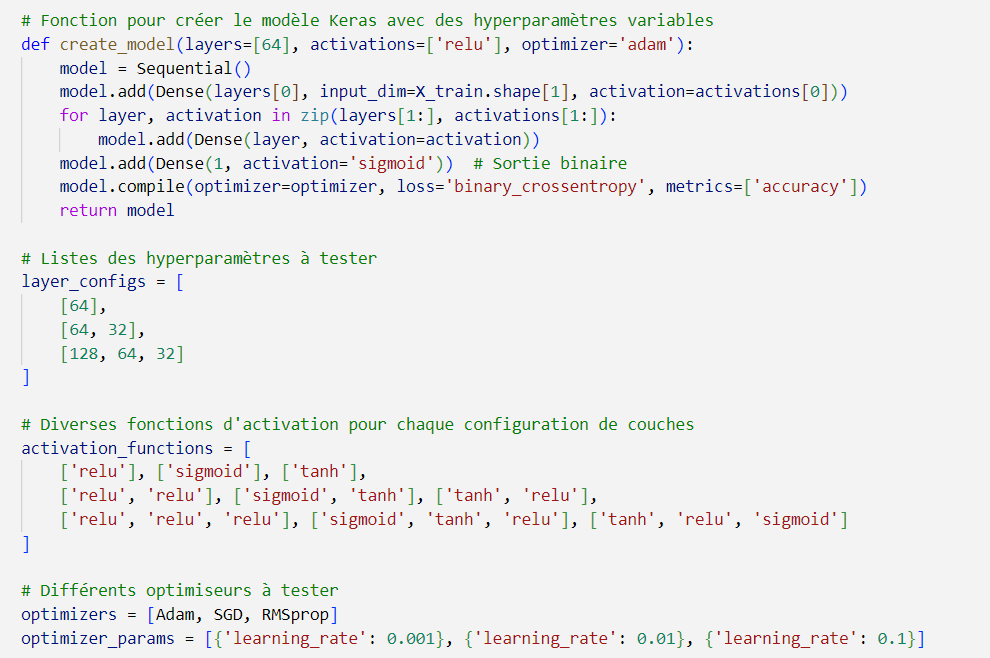
\includegraphics[width=0.9\linewidth]{capture_sas_80.png}
    \caption{Optimisation de l'architecture des couches dans Keras.}
    \label{arch}
\end{figure}

